\chapter{Moving a belief on a grid}
\label{app:gridshift}

The prediction of the grid filter moves the whole belief by the
displacement of one step (\cref{sec:grid}). On a grid this is less simple
than it sounds, because a step is rarely a whole number of cells. This
appendix explains how the code moves the belief, by sharing the mass of
each cell between the cells that its moved copy overlaps, and what that
sharing costs:
a small spread at every step. Notebook~01 runs every example and prints
every number below.

\section{The problem}
\label{sec:gs-problem}

The grid stores one probability per cell: the probability that the
robot is somewhere in that cell. It says nothing about \emph{where} in the
cell, and to move the belief we must decide how to read it. There are two
natural readings:
\begin{itemize}[nosep]
  \item \emph{all the mass at the centre}: the robot is at the centre of
        the cell, with the probability of the cell;
  \item \emph{the mass spread evenly over the cell}: every point of the
        cell is equally likely, that is, inside the cell the position is
        uniformly distributed.
\end{itemize}
Moving the belief by a whole number of cells is easy with either reading:
each cell passes its mass to the cell that many places further on. But
take cells 4 units wide and a step of 4 units at $30^\circ$: the
displacement is $(4\cos30^\circ,\,4\sin30^\circ)=(3.46,\,2)$ units, that
is $0.87$ cell along $x$ and $0.5$ cell along $y$, and the moved mass no
longer fits the cells.

\emph{The first reading leads to rounding.}

If all the mass of a cell sits at its centre, the move takes it to one
point, which is not the centre of any cell, and the simplest answer is to
put all the mass in the cell where that point lands. Take cell $0$, the interval $[0,1)$ in units of cells, with its
mass at the centre $0.5$, and a move of $0.87$ cell. The mass should be at
$0.5+0.87=1.37$, which lies in cell $1$, $[1,2)$. Putting the mass in
cell $1$ puts it at the centre $1.5$ of that cell: the mass has moved by
$1$ cell instead of $0.87$. The displacement has been \emph{rounded}, and
the rounding error, $0.13$ cell, is made again at every step, always in
the same direction. After 10 steps the belief has moved $10$ cells
instead of $8.7$: $1.3$ cells, about $5$ units, too far, while staying as
sharp as a single cell. The filter is wrong and confident
(\cref{fig:gsspread}c). The second reading avoids this, as the next
section shows.

\section{Sharing in one dimension}
\label{sec:gs-1d}

Take now the second reading: inside a cell, the position is uniformly
distributed. Measure positions in cells, so that the cell $i$ is the
interval $[i,i+1)$, of length $1$, and write the displacement, in cells,
as $k+f$: a whole number $k$ of cells and a fraction $f$ of a cell, with
$0\le f<1$.

\begin{figure}[t]
\centering
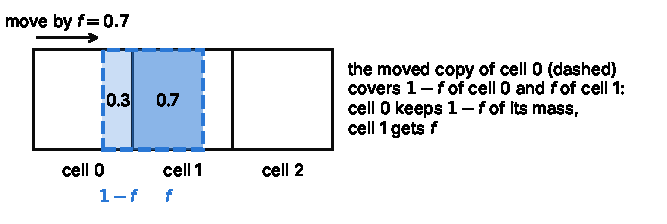
\includegraphics[width=0.8\linewidth]{figures/appF_shift_1d.pdf}
\caption{Where the mass of one cell goes, for a move by $f=0.7$ of a cell
($k=0$). A robot uniform in cell 0 is, after the move, uniform in the
moved copy of cell 0 (dashed), which covers the length $1-f=0.3$ of
cell 0 and $f=0.7$ of cell 1: it is in cell 0 with probability $0.3$ and
in cell 1 with probability $0.7$, and these cells get these fractions of
the mass.}
\label{fig:gs1d}
\end{figure}

\emph{Where can the robot be after the move?} Suppose the robot is in the
cell $i$, at a point $x$ that is uniform on $[i,i+1)$. After the move it
is at $x+k+f$, which is uniform on the moved interval
$[i+k+f,\,i+k+1+f)$: the dashed copy of the cell in
\cref{fig:gs1d}, where $k=0$. That interval does not fit one cell: its
part $[i+k+f,\,i+k+1)$, of length $1-f$, lies in the cell $i+k$, and its
part $[i+k+1,\,i+k+1+f)$, of length $f$, lies in the cell $i+k+1$.

\emph{From lengths to probabilities.} For a uniform distribution on an
interval of length $1$, the probability of a part of the interval is its
length. So the robot ends up in the cell $i+k+1$ with probability $f$,
and in the cell $i+k$ with probability $1-f$. This is the only place where
a displacement becomes a probability, and it is the uniform distribution
inside the cell that makes it one. With the mass of the cell $i$, the
cell $i+k$ receives the fraction $1-f$ and the cell $i+k+1$ the fraction
$f$: this is \emph{sharing}. When $k=0$, as for a
step shorter than a cell, the first of the two is the cell $i$ itself,
which keeps $1-f$; when $k\ge1$, the cell $i$ keeps nothing.

\begin{figure}[t]
\centering
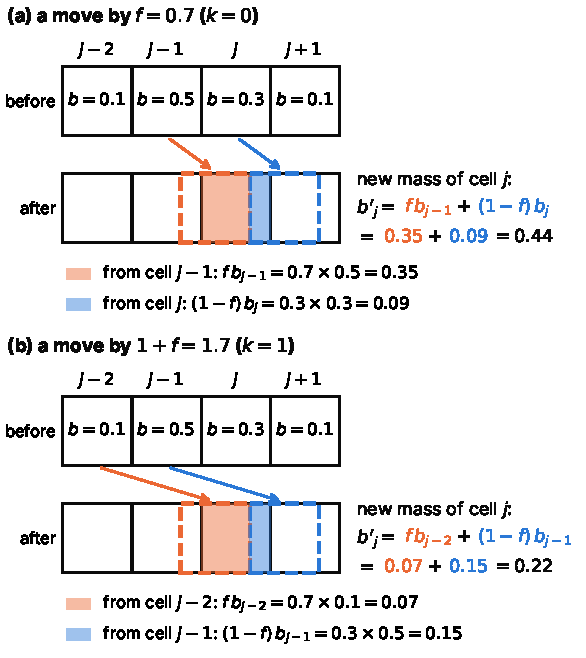
\includegraphics[width=0.72\linewidth]{figures/appF_shift_receive.pdf}
\caption{What one cell receives when all the cells move at once, with
$f=0.7$ and the same belief before the move. (a) $k=0$: cell $j$ is
overlapped by the copy of the cell before it, which covers the fraction
$f$ of it, and by its own copy, which covers the fraction $1-f$; it
receives $0.7\times0.5=0.35$ from cell $j-1$ and $0.3\times0.3=0.09$ from
itself, so its new mass is $0.44$. (b) $k=1$, one more whole cell: the
two copies that overlap cell $j$ come from one cell further back, so cell
$j$ receives $f$ of cell $j-2$ and $1-f$ of cell $j-1$, and its new mass
is $0.7\times0.1+0.3\times0.5=0.22$.}
\label{fig:gsreceive}
\end{figure}

Every cell is moved in this way at the same time. So the new mass of a
cell $j$ is the sum of what it receives (\cref{fig:gsreceive}a for $k=0$,
\cref{fig:gsreceive}b for $k=1$): $1-f$ of the mass of the cell
$j-k$ and $f$ of the mass of the cell $j-k-1$,
\[
  b'_j=(1-f)\,b_{j-k}+f\,b_{j-k-1}.
\]
(This is what is called linear interpolation; the code calls
\code{scipy.ndimage.shift} with \code{order=1}.) Below, the whole number
$k$ plays no role, since moving by whole cells changes neither the
spread nor the error, so the examples take $k=0$.


\emph{The mean is right.} Follow the mass of one cell $i$, with $k=0$.
After the sharing it sits at the cell $i$, with the probability $1-f$,
and at the cell $i+1$, with the probability $f$.
Its average position is
\[
  (1-f)\,i+f\,(i+1)=i+f :
\]
on average, the mass has moved by exactly $f$. Sharing does not drift.

\emph{But the belief is spread.} Before the move, all of this mass was
in one cell; now it is in two. The spread is measured by the variance of
the position, as the grid records it, that is, by its cell. For a
position that takes a few values $x_k$ with the probabilities $p_k$
(adding up to $1$), and has the mean $m=\sum_kp_kx_k$, the variance is the
average of the squared distances to the mean, each weighted by its
probability:
\[
  \Var=\sum_kp_k\,(x_k-m)^2 .
\]
Its square root, the standard deviation $\sigma$, is a typical distance
from the mean, and what it says about probabilities is made precise by
Chebyshev's inequality: the probability that the position $X$ is at
least the distance $a>0$ from the mean is at most $\Var/a^2$,
\[
  \Pr\bigl(|X-m|\ge a\bigr)\le\frac{\Var}{a^2}.
\]
For example, with $a=2\sigma$, and $\Var=\sigma^2$:
$\Pr\bigl(|X-m|\ge2\sigma\bigr)\le\sigma^2/(2\sigma)^2=1/4$; the position
is at least $2\sigma$ from the mean with a probability of at most $1/4$.

Here, following one unit of mass from the cell $i$ (with $k=0$), the
position takes two values: $x_1=i$, with the probability $p_1=1-f$, and
$x_2=i+1$, with the probability $p_2=f$, the probabilities found above.

\emph{Units.} Positions are counted in cells (the cell $i$ is at the
position $i$), so the distances between positions, such as $x_k-m$, and
the displacements, such as $f$, are measured in cells too. A squared
distance is then measured in cells squared, written cell$^2$, and so is
the variance, an average of squared distances; the probabilities have no
unit. The square root of the variance, the standard deviation, is back
in cells. With cells 4 units wide, $1$ cell is $4$ units and
$1$\,cell$^2$ is $16$ units$^2$.

The mean is $m=i+f$ cell:
\begin{center}
\begin{tabular}{cccc}
  \toprule
  position $x_k$ (cell) & probability $p_k$ & $x_k-m$ (cell) & $(x_k-m)^2$ (cell$^2$)\\
  \midrule
  $i$   & $1-f$ & $i-(i+f)=-f$    & $f^2$\\
  $i+1$ & $f$   & $(i+1)-(i+f)=1-f$ & $(1-f)^2$\\
  \bottomrule
\end{tabular}
\end{center}
Multiplying each squared distance by its probability and adding:
\begin{align*}
  \Var&=(1-f)\times f^2\ \text{cell}^2+f\times(1-f)^2\ \text{cell}^2\\
      &=f(1-f)\times\bigl(f+(1-f)\bigr)\ \text{cell}^2
       &&\text{taking out the common factor $f(1-f)$}\\
      &=f(1-f)\ \text{cell}^2 .
\end{align*}
With the numbers of \cref{fig:gs1d}, $f=0.7$: the mean is $0.7$ cell,
the two positions $0$ and $1$ are at the distances $-0.7$ and $0.3$ cell
from it, and
\[
  \Var=0.3\times0.49\ \text{cell}^2+0.7\times0.09\ \text{cell}^2
  =(0.147+0.063)\ \text{cell}^2=0.21\ \text{cell}^2=0.7\times0.3\ \text{cell}^2 .
\]
For $f=0.87$ it is $0.87\times0.13=0.11$\,cell$^2$; its largest value is
$0.25$\,cell$^2$, for $f=0.5$, a standard deviation of half a cell.

\emph{Where the spread comes from.} The move itself spreads nothing: a
robot uniform on the cell $[i,i+1)$ becomes a robot uniform on
$[i+f,i+1+f)$, an interval of the same length. The spread comes from the
next step, when the grid stores the result. It keeps only the
probability of each cell, $1-f$ and $f$, and forgets where inside the cell
that probability lies: the part of length $1-f$, which lay at the end of
the cell $i$, is read again as spread over the whole cell $i$, and the
part of length $f$ over the whole cell $i+1$. That forgetting, made at
every step, is what adds the variance $f(1-f)$. The robot did not become
more uncertain: this spread is an artefact of the grid.

\emph{It adds up over the steps.} Follow now the whole belief, not one
cell, with $k=0$ as above. Let $X$ be the position of the robot before
the shift, counted in cells as the grid records it: $X=j$ with the
probability $b_j$. The sharing can be pictured as a coin tossed for the
robot: a variable $S$ equal to $0$ with probability $1-f$ and to $1$
with probability $f$, the same for every cell, hence independent of $X$;
the robot is then moved to $X+S$. The distribution of $X+S$ is the new
belief:
\begin{align*}
  \Pr(X+S=j)
  &=\Pr(X=j,\,S=0)+\Pr(X=j-1,\,S=1)
  &&\text{the two ways to reach $j$}\\
  &=\Pr(X=j)\Pr(S=0)+\Pr(X=j-1)\Pr(S=1)
  &&\text{$X$ and $S$ independent}\\
  &=(1-f)\,b_j+f\,b_{j-1}=b'_j
  &&\text{the sharing rule.}
\end{align*}
So a shift adds to the position an independent variable $S$. This is
the discrete form of the probabilistic meaning of the convolution
(\cref{sec:grid}): blurring a density by a weight gives the density of a
sum of independent variables; here the weight is $(1-f,\,f)$, the
distribution of $S$.

$S$ takes the values $0$ and $1$ with the probabilities $1-f$ and $f$:
these are the two positions of the table above, with $i=0$, so
$\Var S=f(1-f)$\,cell$^2$. Now the variances of independent variables
add. Write $\tilde X=X-\E X$ and $\tilde S=S-\E S$, whose expectations
are $0$; then $X+S-\E[X+S]=\tilde X+\tilde S$, and
\begin{align*}
  \Var(X+S)
  &=\E\bigl[(\tilde X+\tilde S)^2\bigr]
  &&\text{definition of the variance}\\
  &=\E[\tilde X^2]+2\,\E[\tilde X\tilde S]+\E[\tilde S^2]
  &&\text{expand; linearity of }\E\\
  &=\Var X+2\,\E[\tilde X]\,\E[\tilde S]+\Var S
  &&\text{$\tilde X$ and $\tilde S$ independent}\\
  &=\Var X+f(1-f)
  &&\E[\tilde X]=\E[\tilde S]=0,
\end{align*}
the one-dimensional case of Consequence~2 in \cref{sec:grid}. Each
shift tosses a new coin, independent of the earlier ones and of the
starting position $X_0$: after $t$ shifts the position is
$X_t=X_0+S_1+\dots+S_t$, and, applying this result $t$ times,
\[
  \Var X_t=\Var X_0+t\,f(1-f) .
\]
The sharing adds $f(1-f)$\,cell$^2$ at every shift, and $t\,f(1-f)$
after $t$ shifts. (A whole number $k$ of cells would add $k$ to $S$,
which changes neither its variance nor this result.)
\Cref{fig:gsspread} shows it for $f=0.87$, where
$f(1-f)=0.87\times0.13=0.1131$\,cell$^2$: the belief starts in one cell,
so $\Var X_0=0$, and the variance measured on the grid is $0.1131$ after
one shift and $5\times0.1131=0.5655$\,cell$^2$ after five.

\begin{figure}[t]
\centering
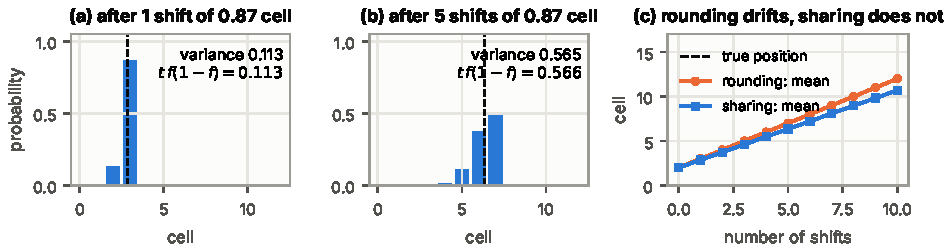
\includegraphics[width=\linewidth]{figures/appF_shift_spread.pdf}
\caption{Repeated shifts by $f=0.87$ cell of a belief that starts in cell
$2$. (a) After one shift the mass is shared between two cells, $0.13$ and
$0.87$; the dashed line is the true position. (b) After five shifts it is
spread over four cells, with the variance $5f(1-f)$. (c) The mean position
over ten shifts: with rounding (each mass goes to the nearest cell centre)
the belief moves one cell per step and drifts away from the true position;
with sharing its mean stays on it.}
\label{fig:gsspread}
\end{figure}

\section{Sharing in two dimensions}
\label{sec:gs-2d}

In the plane, a move by the fractions $f_x$ along $x$ and $f_y$ along $y$
translates the old square cell so that it overlaps four cells
(\cref{fig:gs2d}a), and its mass is shared between these four. As in
one dimension, a whole number of cells along each axis is moved first,
and every cell is shared at the same time, so each cell receives
contributions from four cells. The shares are, again, the covered fractions, now
areas. Each overlap is a rectangle whose width is a covered length along
$x$ and whose height is a covered length along $y$:
\begin{center}
\begin{tabular}{lcc}
  \toprule
  & left column & right column\\
  \midrule
  top row    & $(1-f_x)\,f_y$ & $f_x\,f_y$\\
  bottom row & $(1-f_x)(1-f_y)$ & $f_x(1-f_y)$\\
  \bottomrule
\end{tabular}
\end{center}
The four areas add up to $1$: the translated square has the area $1$.
In two dimensions, too, this is what the code does, with the same call
as in one dimension; notebook~01 checks it for $f_x=0.87$ and
$f_y=0.5$.

\begin{figure}[t]
\centering
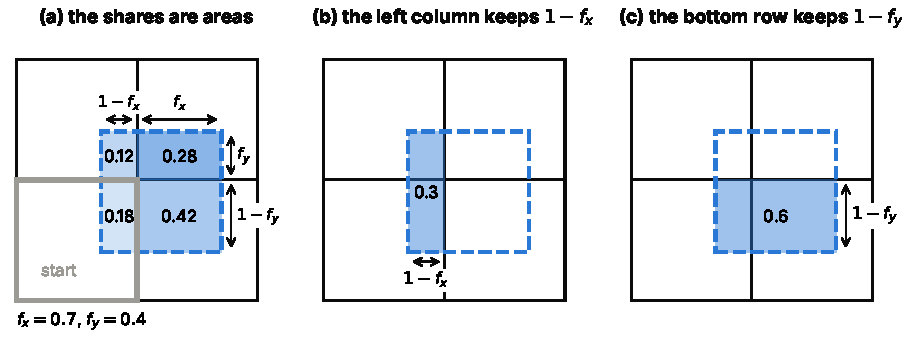
\includegraphics[width=0.75\linewidth]{figures/appF_shift_2d.pdf}
\caption{Sharing in two dimensions. (a) The cell that starts at the bottom
left (grey) is moved by $f_x=0.7$ along $x$ and $f_y=0.4$ along $y$
(dashed). It overlaps four cells, and the shares are the overlapping
areas: $0.18$, $0.42$, $0.12$, $0.28$. (b) The part that falls in the
left column is a strip of width $1-f_x=0.3$ and height $1$: the left
column keeps $1-f_x$ of the mass, whatever $f_y$.}
\label{fig:gs2d}
\end{figure}

\emph{Along each axis, the one-dimensional sharing.} Look only at the
$x$ coordinate. The left column receives the two overlaps on the left:
\[
  (1-f_x)(1-f_y)+(1-f_x)\,f_y=(1-f_x)\bigl((1-f_y)+f_y\bigr)=1-f_x ,
\]
taking out the common factor $1-f_x$. Geometrically, the part of the
translated square that lies in the left column is a strip of width $1-f_x$
and height $1$ (\cref{fig:gs2d}b), whose area is $1-f_x$. Likewise the
right column receives $f_x$. So, along $x$, the mass is shared exactly as
in one dimension, with the fraction $f_x$, and the sharing adds the
variance $f_x(1-f_x)$ along $x$. In the same way it adds $f_y(1-f_y)$
along $y$.

\emph{The example of \cref{sec:gs-problem}.} For the step at $30^\circ$,
$f_x=0.87$ and $f_y=0.5$, and each prediction adds the variances
$0.87\times0.13=0.11$\,cell$^2$ along $x$ and $0.5\times0.5=0.25$\,cell$^2$
along $y$, on top of the motion noise. A step along an axis, $(4,0)$
units, is exactly one cell: $f_x=f_y=0$, and the sharing adds nothing.

\section{What it means for the filter}
\label{sec:gs-filter}

Each prediction of the grid filter widens the belief by the motion noise
and, unless the step is a whole number of cells, by the sharing as well:
up to $0.25$\,cell$^2$ per axis, against the motion noise of about $0.4$
units, a tenth of a cell 4 units wide. Notebook~01 starts a grid belief in
a single cell and predicts 50 times without update: with the heading along
an axis its spread is $2.5$ units, close to the $2.0$ of the motion noise
alone; with the heading at $30^\circ$ it is $12.4$ units. The filter is
therefore more cautious than the model: it never claims a precision that
the grid cannot represent. Between updates this is harmless, since a
measurement soon narrows the belief again; but a grid filter predicting
over many steps without measurements spreads faster than it should.

Two remedies exist. Smaller cells reduce the spread in units, since it is
at most half a cell. Or the filter can move the belief by whole cells only,
and keep the leftover fraction of the displacement for the next step:
the mass is then never shared, and, because the leftover is carried
forward instead of being dropped, the position error stays below half a
cell instead of accumulating as in \cref{sec:gs-problem}.
